\part{Evaluando los algoritmos de scheduling}

\section{Ejercicio 6}

Implementamos el tipo de tarea TaskBatch que recibe como par\'ametro \verb|tot| (tiempo total de ejecuci\'on) y \verb|blocks| (cantidad de bloqueos).

\begin{framed}
\begin{verbatimtab}
void TaskBatch(vector<int> params) {
	int tot = params[0];
	int blocksC = params[1];
	
	// INICIALIZAMOS SEMILLA DE RAND()
	srand ( time(NULL) );
	
	vector<bool> blocks = vector<bool>(tot-1);
	for(int i=0;i<blocksC;i++) {
		int blockT = rand()%(blocks.size()-1);
		if( !blocks[blockT] )
			blocks[blockT] = true;
		else
			i--;
	}
	for(int i=0;i<(int)blocks.size();i++) {
		if( blocks[i] )
			uso_IO(1);
		else
			uso_CPU(1);
	}
}
\end{verbatimtab}
\end{framed}

\section{Ejercicio 7}

Primero pensamos que medidas afectar\'ian a un scheduler que procese tareas de tipo Batch.

Pensamos el mas dedidas importantes para un sistema batch.

Eficiencia: tratar de que la CPU este ``ocupada'' todo el tiempo.\\
Carga del sistema: minimizar la cant. de procesos listos que esten esperando CPU.\\
Latencia: minimizar el tiempo requerido para que un proceso empiece a dar resultados.\\
Tiempo de ejecucion: minimizar el tiempo total que le toma a un proceso ejecutar completamente.

\section{Ejercicio 8}

\subsection{(a) Starvation}

En este algoritmo, es posible que una tarea TaskCPU 20 sufra inanici\'on f\'acilmente en el siguiente esquema:

Procesos:
\begin{itemize}
 \item Una Tarea TaskCPU 20
 \item Dos tareas en el tiempo @1 que esten constantemente haciendo entrada/salida.
\end{itemize}

Colas:
\begin{itemize}
 \item Una cola para procesos interactivos
 \item Una cola para procesos con mucha carga de CPU
\end{itemize}

Archivo de procesos:

\begin{framed}
\begin{verbatim}
# FILE ejercicio8_a.tsk
TaskCPU 20
@1
*2 TaskIOMultiple 20
\end{verbatim}
\end{framed}

Invocaci\'on:

\begin{framed}
\begin{verbatim}
./simusched ejercicio8_a.tsk 1 SchedMFQ 2 5 | python graphsched.py > ejercicio8_a.png
\end{verbatim}
\end{framed}

\begin{figure}[h!]
  \caption{Ejemplo de Inanici\'on.}
  \centering
    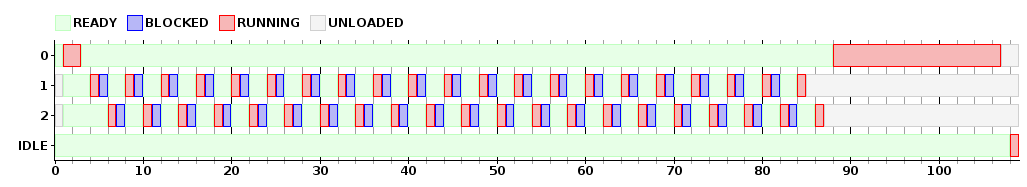
\includegraphics[width=1\textwidth]{img/ejercicio8_a.png}
\end{figure}

\subsection{(b) Ejemplo de Multicolas}

Aca generamos un ejemplos con tres tareas, cada una con un tipo de comportamiento diferente.

\begin{itemize}
 \item Una tarea de uso intensivo de CPU (TaskCPU 60)
 \item Una tarea de tipo Batch con relativamente poca entrada/salida (TaskBatch 50 3)
 \item Una tarea de tipo cliente interactiva, - simulada por una tarea que hace constantemente IO (TaskIOMultiple 15)
\end{itemize}

Luego ejecutamos los tres procesos en un scheduler MFQ con tres colas de pioridad (2 5 10)

\begin{framed}
\begin{verbatim}
# FILE ejercicio8_b.tsk
TaskCPU 60
TaskBatch 50 3
TaskIOMultiple 15
\end{verbatim}
\end{framed}

Invocaci\'on:

\begin{framed}
\begin{verbatim}
./simusched ejercicio8_b.tsk 1 SchedMFQ 2 5 10 | python graphsched.py > ejercicio8_b.png
\end{verbatim}
\end{framed}

El resultado fue el siguiente:

\begin{figure}[h!]
  \caption{Ejemplo de MFQ - como los porcesos van cambiando de cola de pioridad.}
  \centering
    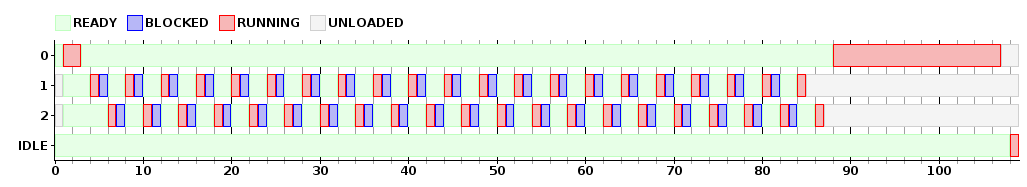
\includegraphics[width=1\textwidth]{img/ejercicio8_a.png}
\end{figure}

